\documentclass[a4paper,14pt]{article}
\usepackage[left=2cm,right=2cm, top=2cm,bottom=2cm, bindingoffset=0cm]{geometry}
\usepackage[T2A]{fontenc}
\usepackage[utf8]{inputenc}
\usepackage[english,russian]{babel}
\usepackage{amsmath,amsfonts,amssymb,amsthm,mathtools,graphicx}
\usepackage{fancybox,fancyhdr}
\usepackage{tabularx}
\usepackage{multirow}
\usepackage{bigstrut}
\usepackage{booktabs}
\usepackage{float}
\usepackage{xcolor}
\usepackage{array}
\usepackage{caption}

\DeclareGraphicsExtensions{.pdf,.png,.jpg}

\author{Ануфриев Андрей}
\title{Лабораторная работа № 3.10 \\ Изучение свободных затухающих электромагнитных колебаний}
\date{01.04.2026}

\begin{document}

    \begin{figure}[h]
        \centering
        \begin{minipage}{0.45\linewidth}
            \centering
            
\includegraphics[width=\linewidth]{slogan_chernyy.png}
            \label{fig:slogan}
        \end{minipage}
        \hfill
        \begin{minipage}{0.45\linewidth}
            \centering
            
\includegraphics[width=\linewidth]{cs-logo.png}
            \label{fig:logo}
        \end{minipage}
    \end{figure}
    \begin{table}[htbp]
        \centering
        \begin{tabular}{lrlr}
            Группа & \qquad \qquad P3219 & К работе допущен & \qquad \qquad \qquad \qquad \qquad \qquad \\
            \cmidrule{2-2}\cmidrule{4-4}
            Студент &  \qquad \qquad Торопов П.К.  & Работа выполнена & \qquad \qquad \qquad \qquad \qquad \qquad \\
            \cmidrule{2-2}\cmidrule{4-4}
            Преподаватель & \qquad \qquad Коробков М.П. & Отчет принят & \qquad \qquad \qquad \qquad \qquad \qquad \\
            \cmidrule{2-2}\cmidrule{4-4}
        \end{tabular}%
    \end{table}%
    \vspace{2cm}
    \begin{center}
        \LARGE
        Отчет по лабораторной работе № 3.10 \\
        Изучение свободных затухающих электромагнитных колебаний
    \end{center}
    \vspace{13cm}
    \begin{center}
        2026 год
    \end{center}
    \newpage

% ===== ЦЕЛИ =====
\section{Цели работы}

\begin{enumerate}
    \item Изучить характеристики свободных затухающих колебаний в RLC-контуре.
    \item По экспериментальным данным определить логарифмический декремент затухания $\lambda$, добротность $Q$, собственное сопротивление контура $R_0$.
    \item По зависимости $\lambda(R_M)$ оценить индуктивность катушки $L$ и сравнить с паспортным значением.
    \item Сопоставить экспериментальные и теоретические периоды колебаний при разных $R_M$ и разных емкостях $C$.
\end{enumerate}

% ===== РАБОЧИЕ ФОРМУЛЫ =====
\section{Рабочие формулы и теоретические сведения}

Использованы соотношения из методических указаний:
\begin{equation}
\lambda = \frac{1}{n}\ln\left(\frac{U_i}{U_{i+n}}\right),
\end{equation}
\begin{equation}
Q = \frac{\pi}{\lambda},
\end{equation}
\begin{equation}
R = R_M + R_0,
\end{equation}
\begin{equation}
\lambda \approx \pi R\sqrt{\frac{C}{L}}\quad (\text{для малых сопротивлений}),
\end{equation}
\begin{equation}
T = \frac{2\pi}{\sqrt{\dfrac{1}{LC}-\dfrac{R^2}{4L^2}}},
\end{equation}
\begin{equation}
R_{\text{кр}} = 2\sqrt{\frac{L}{C}}.
\end{equation}

В исходной таблице столбец $T$ соответствует интервалу для $n$ периодов, поэтому при обработке использовался период одного колебания:
\begin{equation}
T_{\text{период}} = \frac{T}{n}.
\end{equation}


% ===== ИЗМЕРИТЕЛЬНЫЕ ПРИБОРЫ =====
\section{Измерительные приборы и установка}

Использованы блок генератора напряжений, осциллограф и учебный стенд с катушкой индуктивности и набором конденсаторов.

По файлу измерений использованы параметры:
\begin{itemize}
    \item $L_{\text{ном}} = 10$ мГн ($\pm 10\%$),
    \item $C_1 = 0.022$ мкФ,
    \item $C_2 = 0.033$ мкФ,
    \item $C_3 = 0.047$ мкФ,
    \item $C_4 = 0.47$ мкФ.
\end{itemize}

% ===== РЕЗУЛЬТАТЫ ИЗМЕРЕНИЙ =====
\section{Результаты прямых измерений и расчёт зависимостей}

Данные обработаны скриптом \texttt{process\_lab\_3\_10.py}. Для каждой строки измерений рассчитаны $\lambda$, $Q$, $R$ и (для участка $R_M \le 100$ Ом при $C_1$) значение $L$.

Для начального участка графика $\lambda(R_M)$ (при $C_1$ и $R_M\le100$ Ом) получена линейная аппроксимация:
\[
\lambda = kR_M + b,
\]
где
\[
k = 0.00500\ \text{Ом}^{-1}, \quad b = 0.324.
\]

Абсцисса точки $\lambda=0$:
\[
R_{M0} = -\frac{b}{k} = -64.77\ \text{Ом},
\]
откуда собственное сопротивление контура:
\[
R_0 = -R_{M0} = 64.77\ \text{Ом}.
\]

% ===== БЛОК ВЫЧИСЛЕНИЙ =====
\subsection*{Основные расчётные соотношения}

По формуле малых затуханий получены значения индуктивности на участке $R_M\le100$ Ом; среднее значение:
\[
L_{\text{ср}} = (8.68 \pm 0.24)\ \text{мГн}.
\]

Сравнение с номиналом стенда:
\[
L_{\text{ном}} = 10.0\ \text{мГн},\quad
\left|\frac{L_{\text{ср}}-L_{\text{ном}}}{L_{\text{ном}}}\right|\cdot100\% \approx 13.2\%.
\]

Примеры рассчитанной добротности (для $C_1$):
\begin{itemize}
    \item при $R_M=0$ Ом: $\lambda=0.353$, $Q=8.91$;
    \item при $R_M=100$ Ом: $\lambda=0.860$, $Q=3.65$;
    \item при $R_M=400$ Ом: $\lambda=2.303$, $Q=1.36$.
\end{itemize}

% ===== ОБРАБОТКА =====
\section{Обработка результатов}

\subsection{График $\lambda(R_M)$ и определение $R_0$}

\begin{figure}[H]
\centering
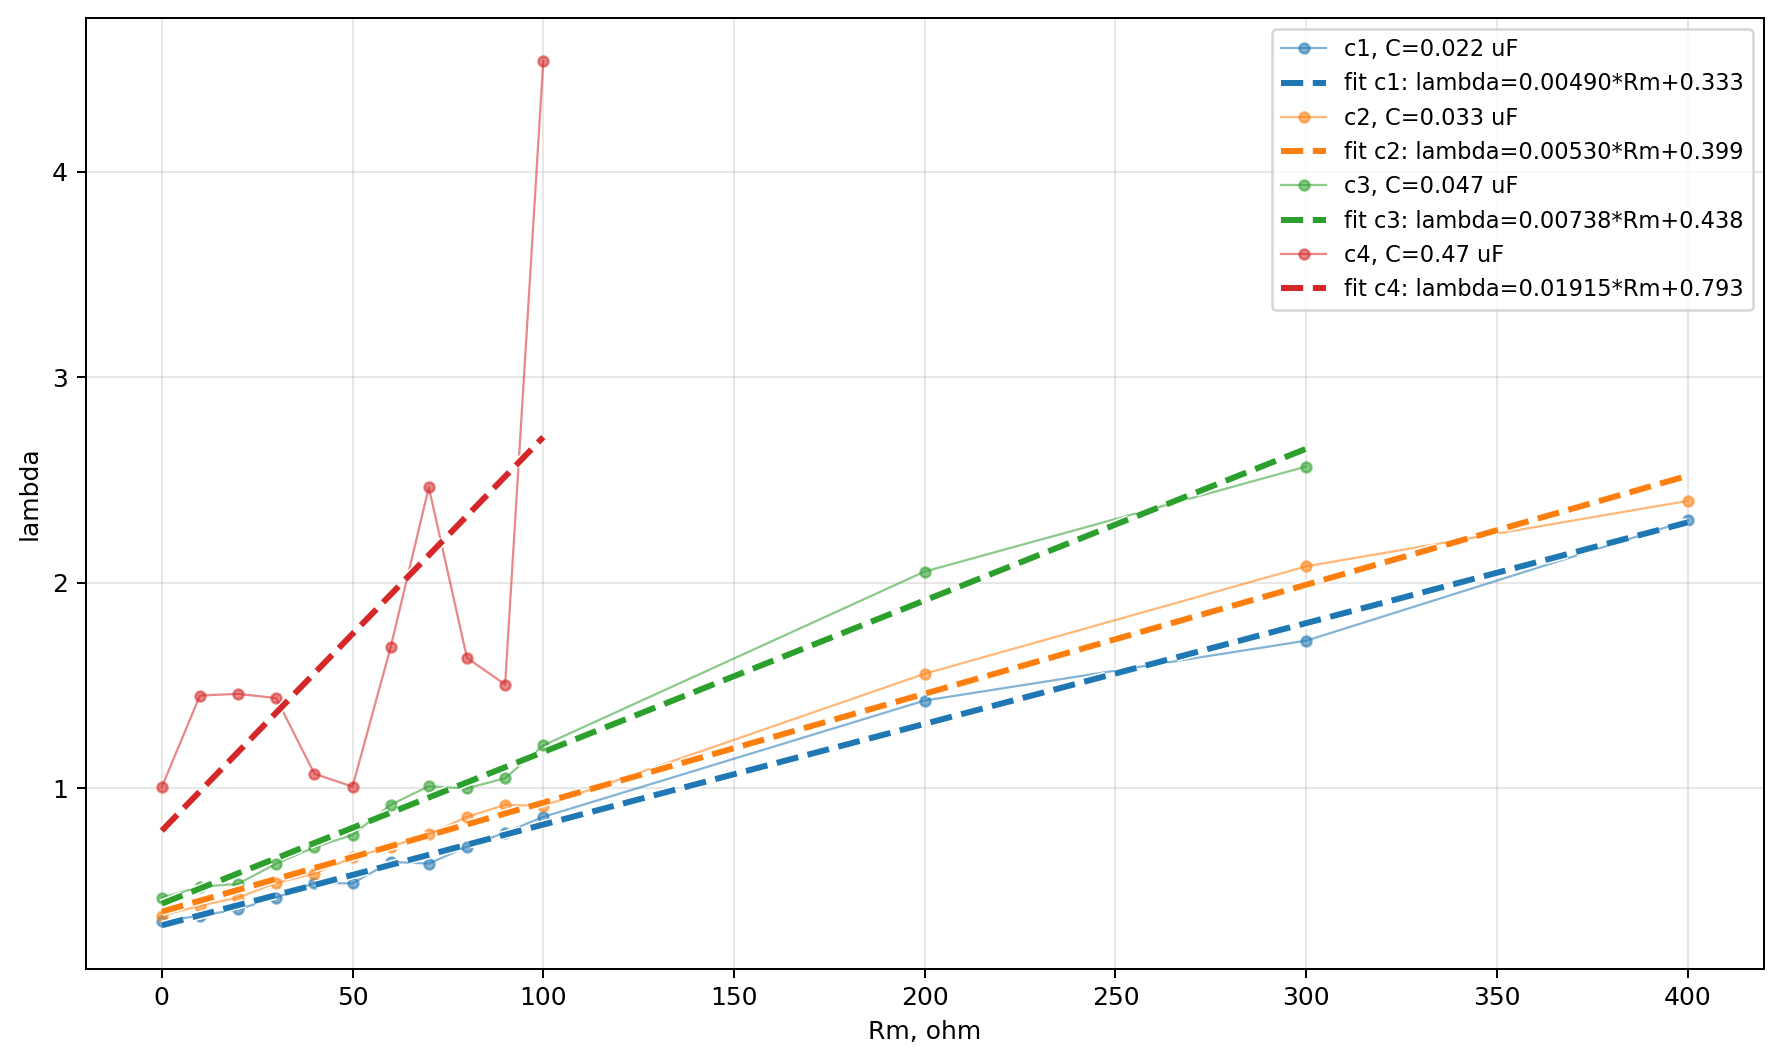
\includegraphics[width=0.9\textwidth]{plot_lambda_vs_rm.png}
\caption{Зависимость логарифмического декремента затухания от сопротивления магазина с линейной аппроксимацией (для $C_1$, $R_M\le 100$ Ом)}
\label{fig:lambda_rm}
\end{figure}

По начальному линейному участку аппроксимация имеет вид
\[
\lambda(R_M) = 0.00500\,R_M + 0.324,
\]
и даёт значение $R_0=64.77$ Ом.

\subsection{Сравнение периода при $C_1$ (точки $R_M=0,200,400$ Ом)}

\begin{table}[H]
\centering
\caption{Сравнение $T_{\text{эксп}}$ и $T_{\text{теор}}$ для $C_1$}
\small
\begin{tabular}{|c|c|c|c|c|}
\hline
$R_M$, Ом & $R$, Ом & $T_{\text{эксп}}$, мс & $T_{\text{теор}}$, мс & $\delta_T$, \% \\
\hline
0   & 64.77  & 0.0910 & 0.0870 & 4.65 \\
200 & 264.77 & 0.0935 & 0.0888 & 5.25 \\
400 & 464.77 & 0.0930 & 0.0935 & 0.50 \\
\hline
\end{tabular}
\end{table}

Расхождения не превышают $\sim5\%$, что соответствует ожидаемой точности эксперимента.

\subsection{Зависимость добротности от полного сопротивления}

\begin{figure}[H]
\centering
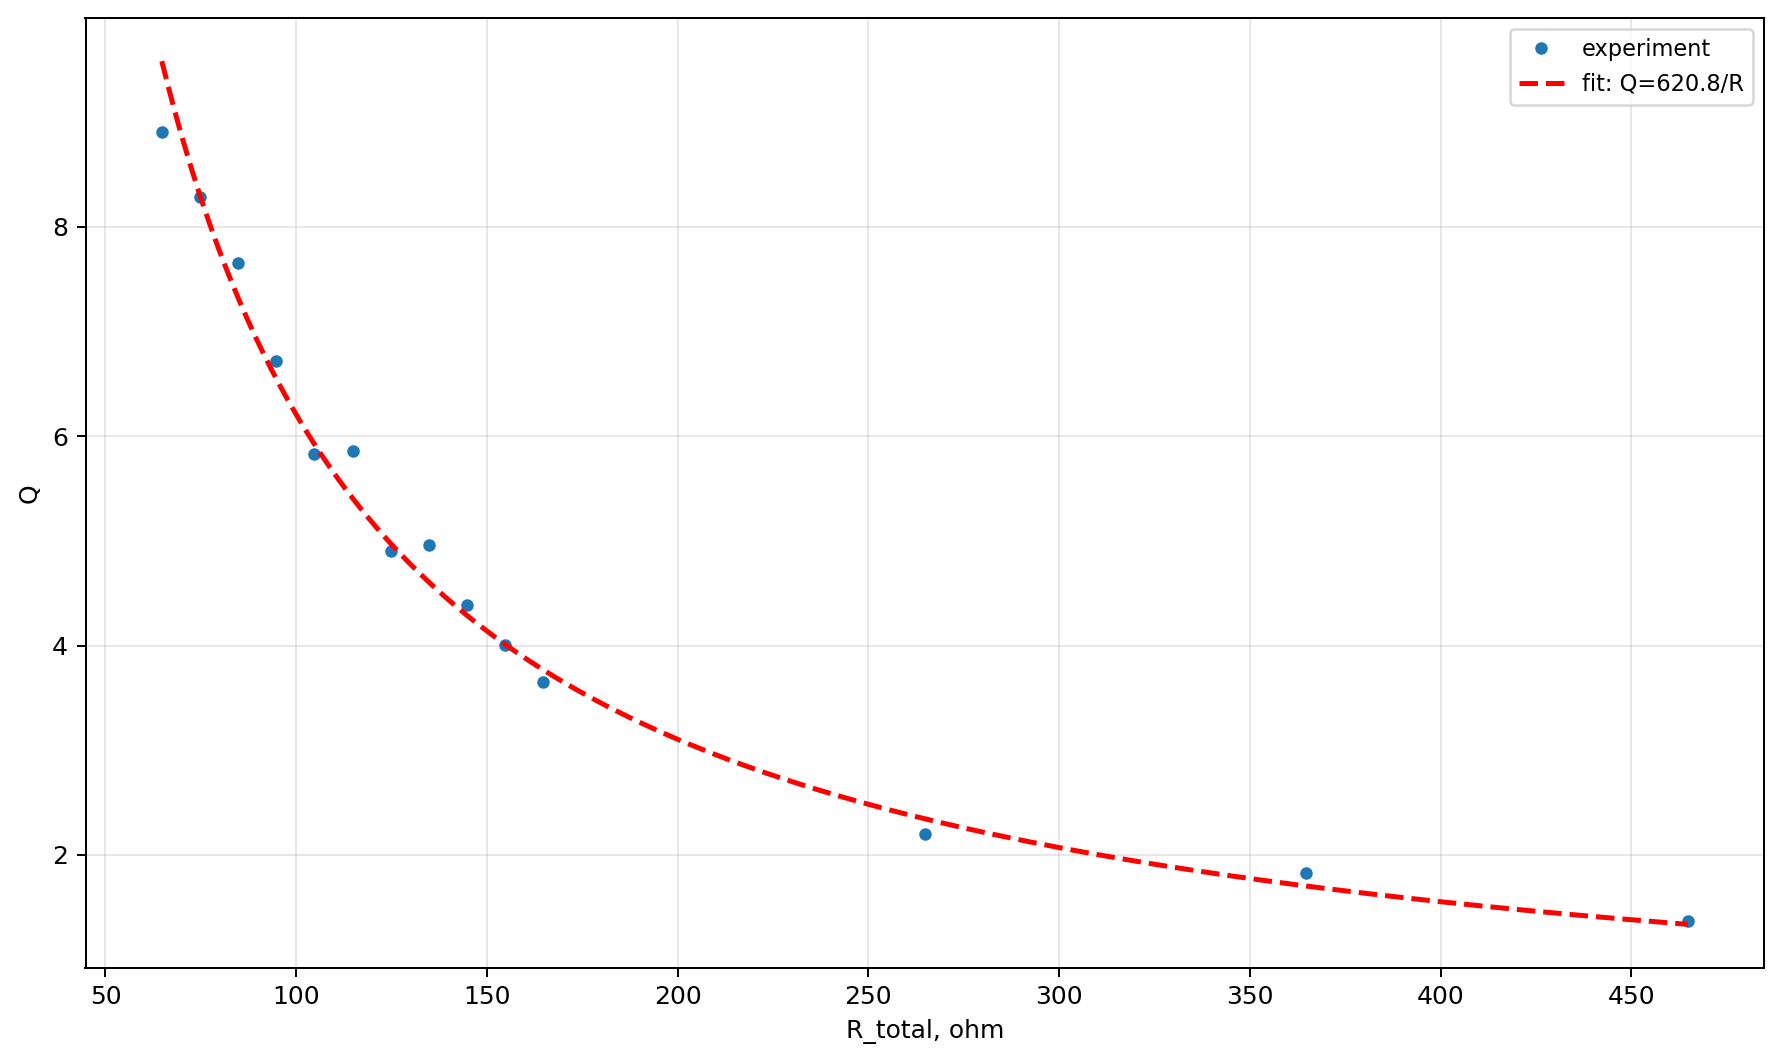
\includegraphics[width=0.9\textwidth]{plot_q_vs_r_total.png}
\caption{Зависимость добротности контура от полного сопротивления (для $C_1$) с аппроксимацией $Q=A/R$}
\label{fig:q_r}
\end{figure}

Для данных $C_1$ добавлена аппроксимация вида
\[
Q(R) = \frac{A}{R},\qquad A \approx 620.8,
\]
что отражает ожидаемую обратную пропорциональность добротности полному сопротивлению.

\subsection{Схематическая реконструкция самих колебаний}

Дополнительно построены временные зависимости, восстановленные по измеренным параметрам:
для напряжения использована модель
\[
U(t)=U_0 e^{-\beta t}\cos(\omega t),\quad \beta=\frac{\lambda}{T_{\text{период}}},\quad \omega=\frac{2\pi}{T_{\text{период}}}.
\]

\begin{figure}[H]
\centering
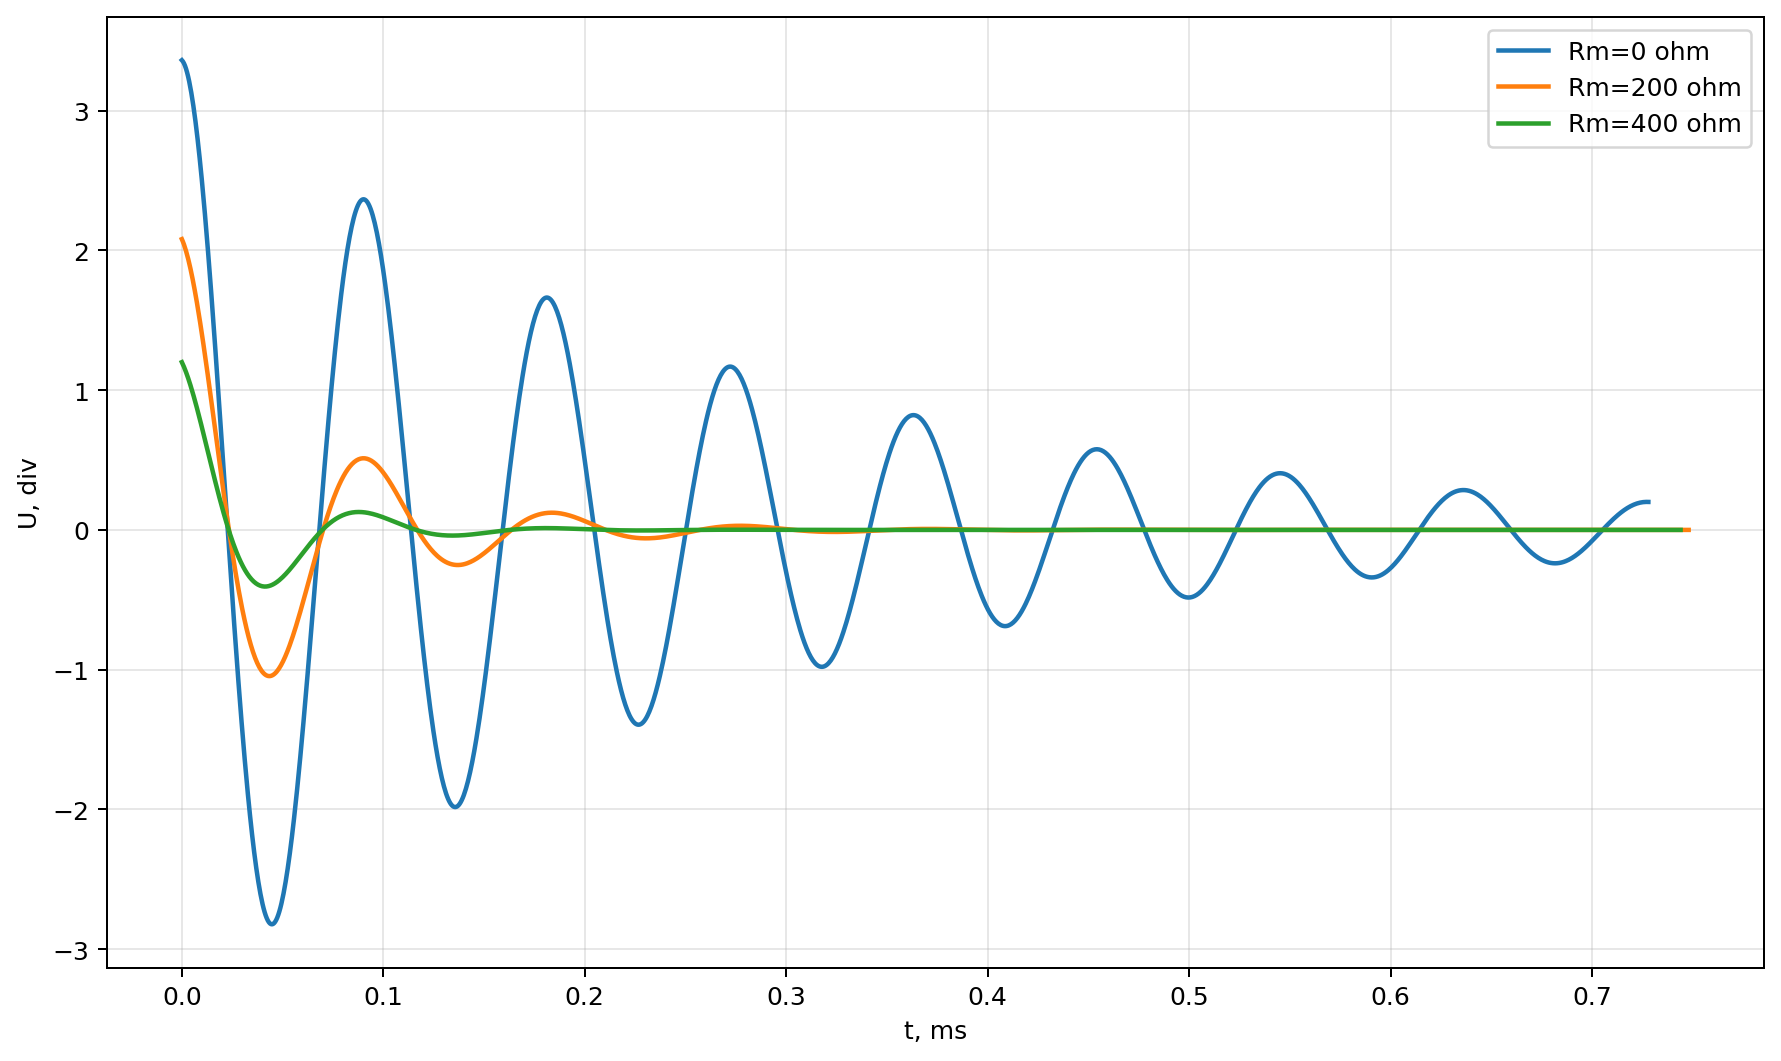
\includegraphics[width=0.9\textwidth]{plot_u_t_reconstructed_c1.png}
\caption{Схематически восстановленные затухающие колебания напряжения $U(t)$ для $C_1$ при разных $R_M$}
\label{fig:u_t_reconstructed}
\end{figure}

Также построен схематический график одновременных колебаний напряжения и тока (в нормированном виде):
\[
\frac{U(t)}{U_0}=e^{-\beta t}\cos(\omega t),
\qquad
\frac{I(t)}{I_0}=e^{-\beta t}\cos(\omega t+\delta),
\]
где фазовый сдвиг $\delta$ вычислялся по теоретическим соотношениям для затухающего контура.

\begin{figure}[H]
\centering
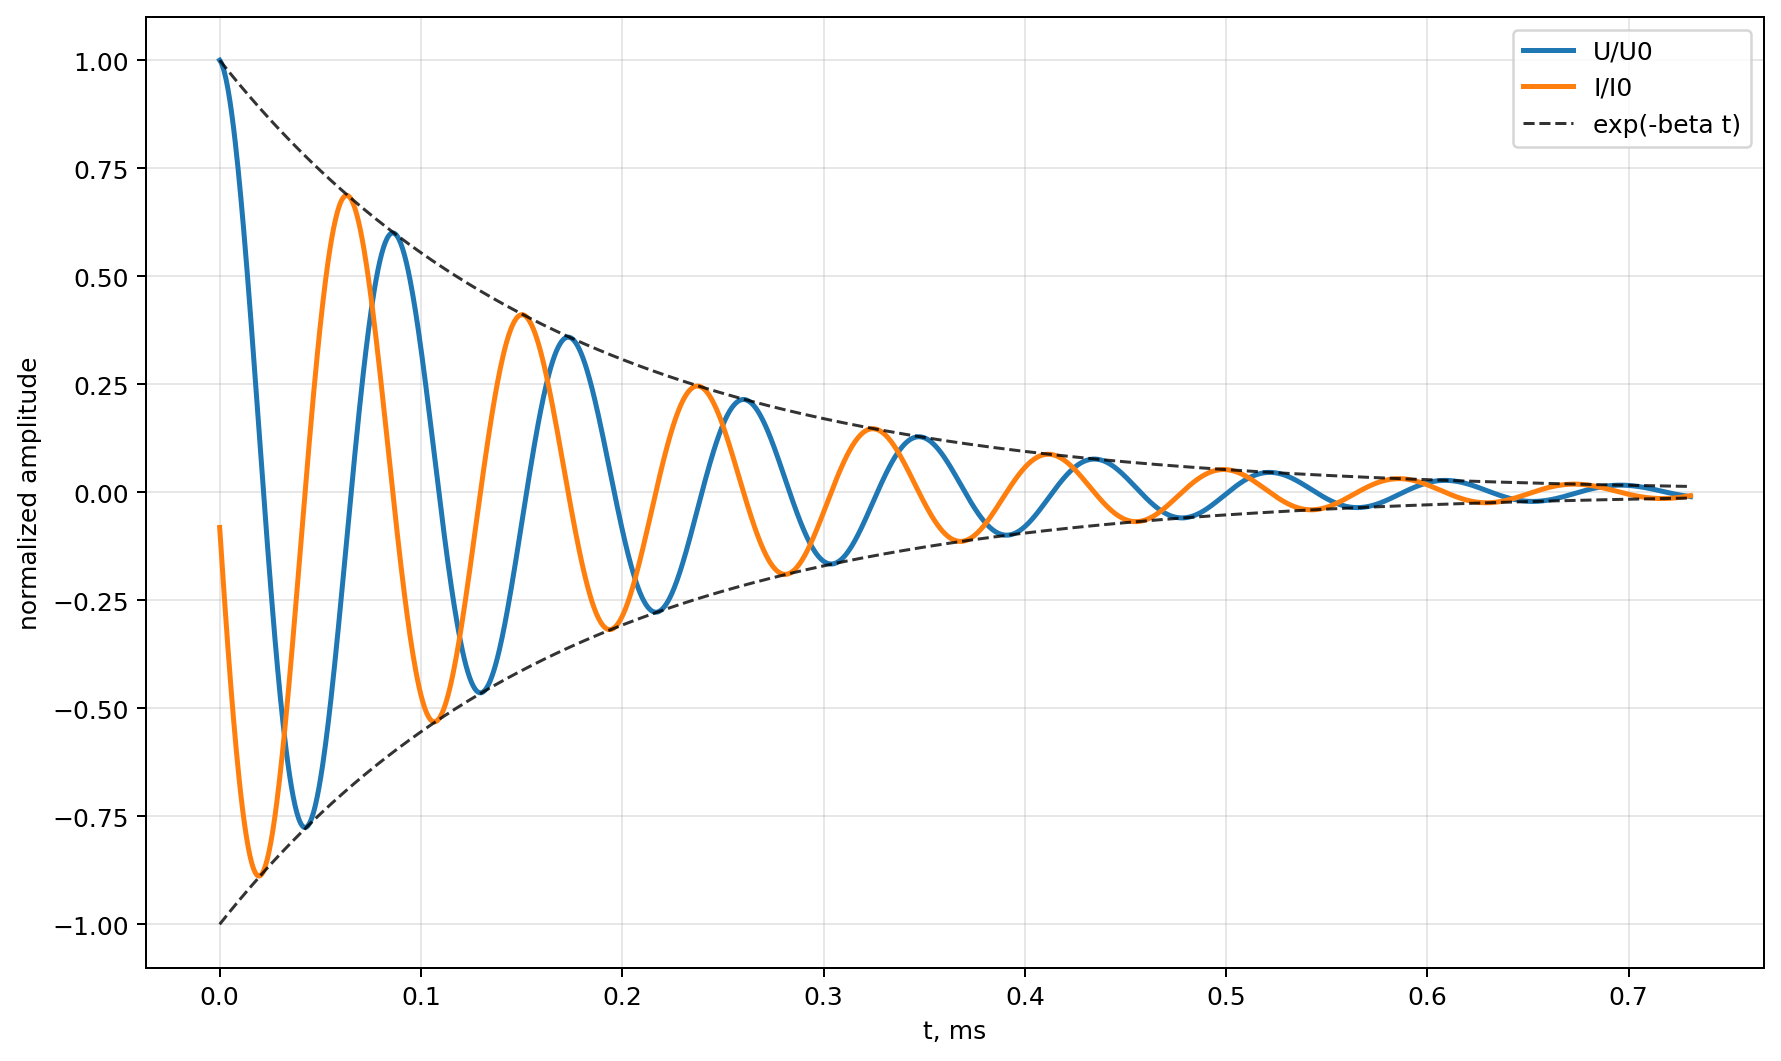
\includegraphics[width=0.9\textwidth]{plot_ui_t_reconstructed_c1.png}
\caption{Схематическая реконструкция колебаний $U(t)$ и $I(t)$ со сдвигом фаз (для $C_1$, $R_M=40$ Ом)}
\label{fig:ui_t_reconstructed}
\end{figure}

Полученные графики корректно отражают физическую картину: при увеличении сопротивления затухание усиливается, а ток опережает напряжение по фазе.

\subsection{Сравнение периодов при разных емкостях}

\begin{table}[H]
\centering
\caption{Сравнение периодов при $R_M=0$ для разных $C$}
\small
\begin{tabular}{|c|c|c|c|}
\hline
$C$, мкФ & $T_{\text{эксп}}$, мс & $T_{\text{теор}}$, мс & $\delta_T$, \% \\
\hline
0.022 & 0.0910 & 0.0870 & 4.65 \\
0.033 & 0.1113 & 0.1066 & 4.40 \\
0.047 & 0.1300 & 0.1273 & 2.13 \\
0.470 & 0.4233 & 0.4133 & 2.43 \\
\hline
\end{tabular}
\end{table}

\begin{figure}[H]
\centering
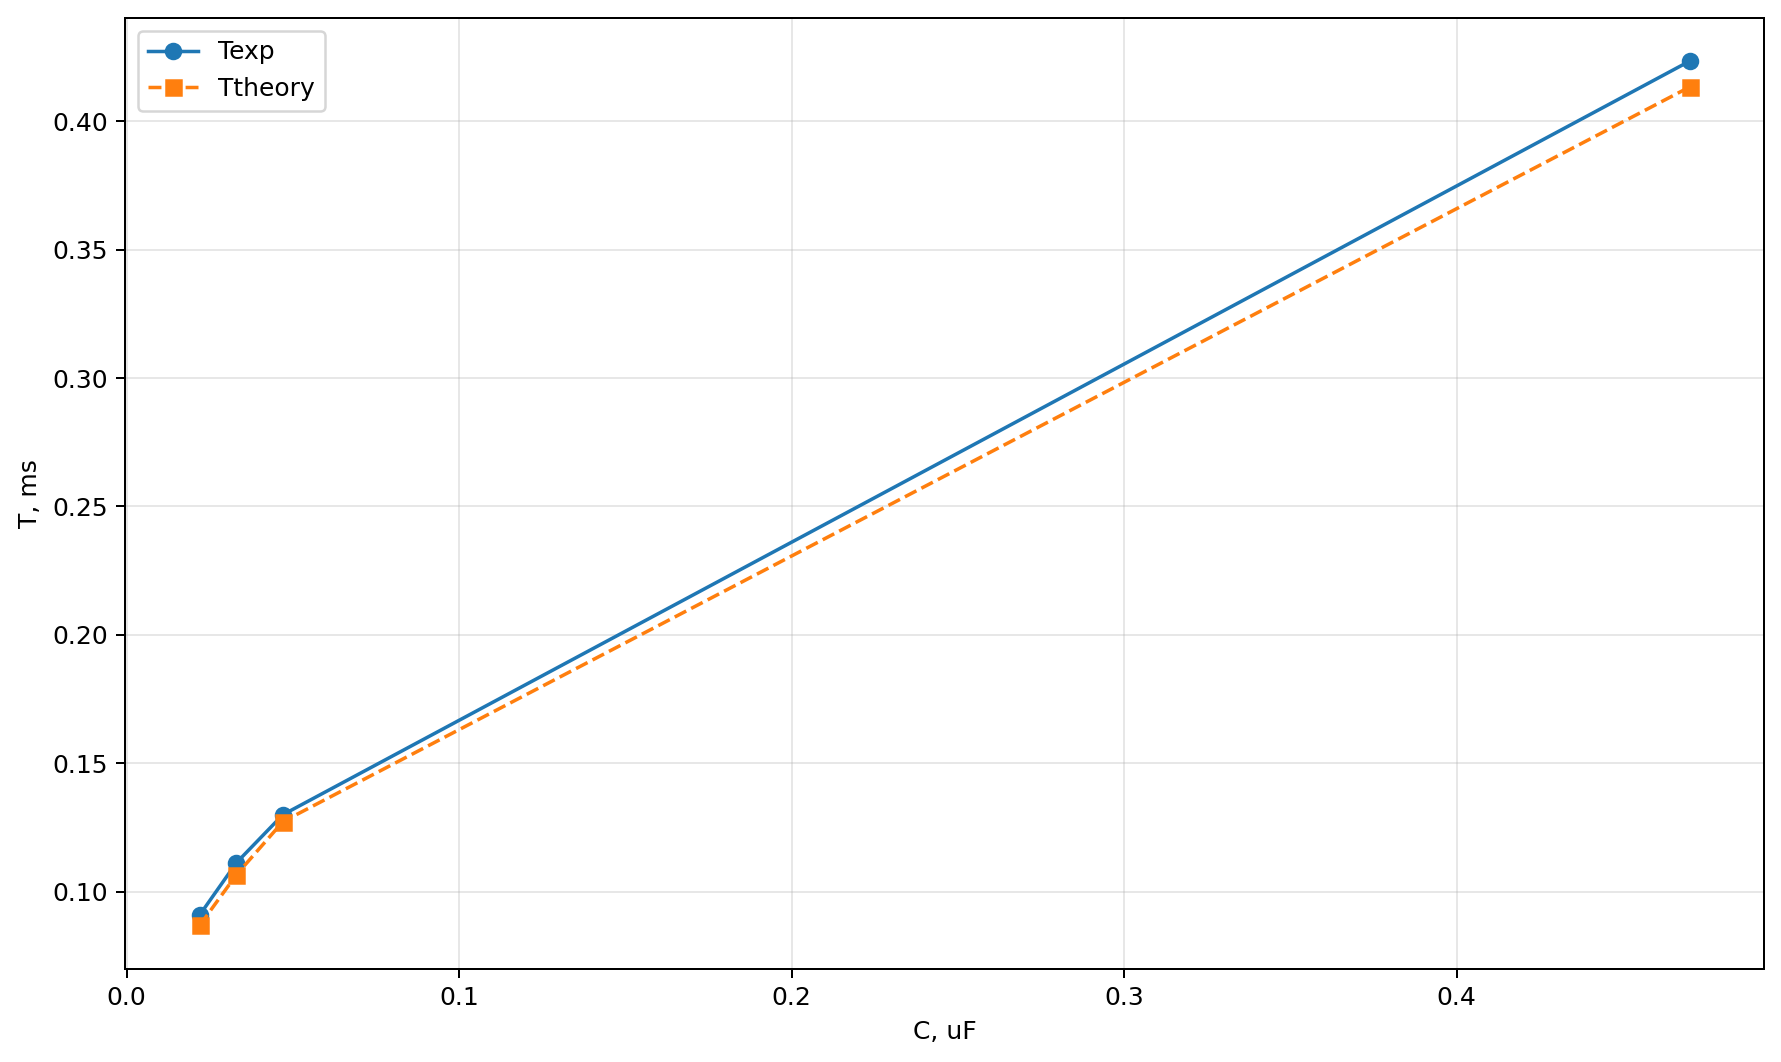
\includegraphics[width=0.9\textwidth]{plot_period_vs_c.png}
\caption{Зависимости $T_{\text{эксп}}(C)$ и $T_{\text{теор}}(C)$ при $R_M=0$}
\label{fig:t_c}
\end{figure}

Среднее относительное расхождение для таблицы выше составляет около $3.4\%$.


% ===== ИТОГОВЫЕ РЕЗУЛЬТАТЫ =====
\section{Итоговые результаты}

\begin{table}[H]
\centering
\small
\begin{tabular}{|l|c|}
\hline
Параметр & Значение \\
\hline
Собственное сопротивление контура $R_0$ & $64.77$ Ом \\
Средняя индуктивность $L_{\text{ср}}$ & $(8.68 \pm 0.24)$ мГн \\
Номинальная индуктивность стенда & $10.0$ мГн \\
$R_{\text{кр, теор}}$ для $C_1$ & $1256.4$ Ом \\
$R_{\text{кр, теор}}$ для $C_4$ & $271.8$ Ом \\
$R_{\text{кр, эксп}}$ (по отметке для $C_4$) & $254.8$ Ом \\
\hline
\end{tabular}
\end{table}

Экспериментальная оценка критического сопротивления (по блоку $C_4$) отличается от теоретической примерно на $6.3\%$, что можно считать удовлетворительным совпадением.

% ===== ВЫВОДЫ =====
\section{Выводы}

\begin{enumerate}
    \item По экспериментальным осциллограммам рассчитаны логарифмический декремент затухания $\lambda$ и добротность $Q$ для серии сопротивлений магазина.

    \item По линейной аппроксимации начального участка $\lambda(R_M)$ определено собственное сопротивление колебательного контура: $R_0=64.77$ Ом.

    \item По данным участка малых сопротивлений получено среднее значение индуктивности катушки: $L_{\text{ср}}=(8.68\pm0.24)$ мГн, что по порядку величины согласуется с паспортным $L_{\text{ном}}=10$ мГн.

    \item Сравнение экспериментальных и теоретических периодов показало хорошее согласие: расхождения в таблицах составили около $2$--$5\%$.

    \item Экспериментальная оценка критического сопротивления по данным для $C_4$ близка к теоретической (разница порядка $6\%$), что подтверждает корректность модели затухающих колебаний для исследуемого контура.
\end{enumerate}

\end{document}

